\documentclass[conference]{IEEEtran}

\usepackage{cite}
\usepackage[dvips]{graphicx}
\usepackage[cmex10]{amsmath}
\interdisplaylinepenalty=2500
\usepackage{array}
\usepackage[tight,footnotesize]{subfigure}

% correct bad hyphenation here
\hyphenation{op-tical net-works semi-conduc-tor}

\begin{document}

\title{A Green Approach to a Multi-Protocol Wireless Communications Network}


\author{\IEEEauthorblockN{Travis Collins\IEEEauthorrefmark{1}, Patrick DeSantis\IEEEauthorrefmark{1}, David Vecchiarelli\IEEEauthorrefmark{1},\\ Alexander M. Wyglinski\IEEEauthorrefmark{1}, and Sean McGrath\IEEEauthorrefmark{2}\\ \\}
\IEEEauthorblockA{\IEEEauthorrefmark{1}Department of Electrical and Computer Engineering\\
Worcester Polytechnic Institute, Worcester, MA 01609--2280, USA\\
Email: \{traviscollins,~pdesantis,~davevecc,~alexw\}@wpi.edu\\ \\}
\IEEEauthorblockA{\IEEEauthorrefmark{2}Department of Electronic and Computer Engineering\\
University of Limerick, Limerick, Ireland\\
Email: sean.mcgrath@ul.ie}}


% make the title area
\maketitle


\begin{abstract}
In this paper, we propose an approach for multiple commercial wireless protocols, focused around mobile networking efficiency.  In addition to evaluating the proposed impact, a hardware prototype was also constructed validating the network approach a single mobile device to intelligently alternate between two wireless protocols, in this case ZigBee and Wi-Fi, in order to reduce network interface power consumption.   This work was a practical approach to examine the policies that enable a system to alternate among several networking interfaces, which were chosen because of their complementary characteristics.  The approach focused around commonly used applications in mobile devices such as file transfers, web browsing, streaming media and text messaging.  By using the concepts of sensing and adaptation from cognitive radio, the system monitors and selects the lowest power intensive wireless protocol while still maintaining an acceptable quality of service for the desired application.  Even though performance transparency could not be sacrificed for power efficiency, experimental validation of this network design shows substantial energy savings: more than a 30\% reduction in energy consumption of the wireless interfaces is possible, leading to a substantial increase in the effective battery lifetime of such a mobile device.
\end{abstract}



\section{Introduction}

Today wireless communications are growing at exponential rates, driven primarily by cellphone markets and mobile computing\cite{two}.  According to \cite{three} ``currently 3\% of the world-wide energy is consumed by the ICT (Information \& Communications Technology) infrastructure that causes about 2\% of the world-wide CO2 emissions, which is comparable to the world-wide CO2 emissions by airplanes or one quarter of the world-wide CO2 emissions by cars".  This consumption coupled with battery technology's comparatively stagnant development\cite{five}, alternative power saving strategies must be examined to reduce consumption.  

\begin{figure}
\begin{center}
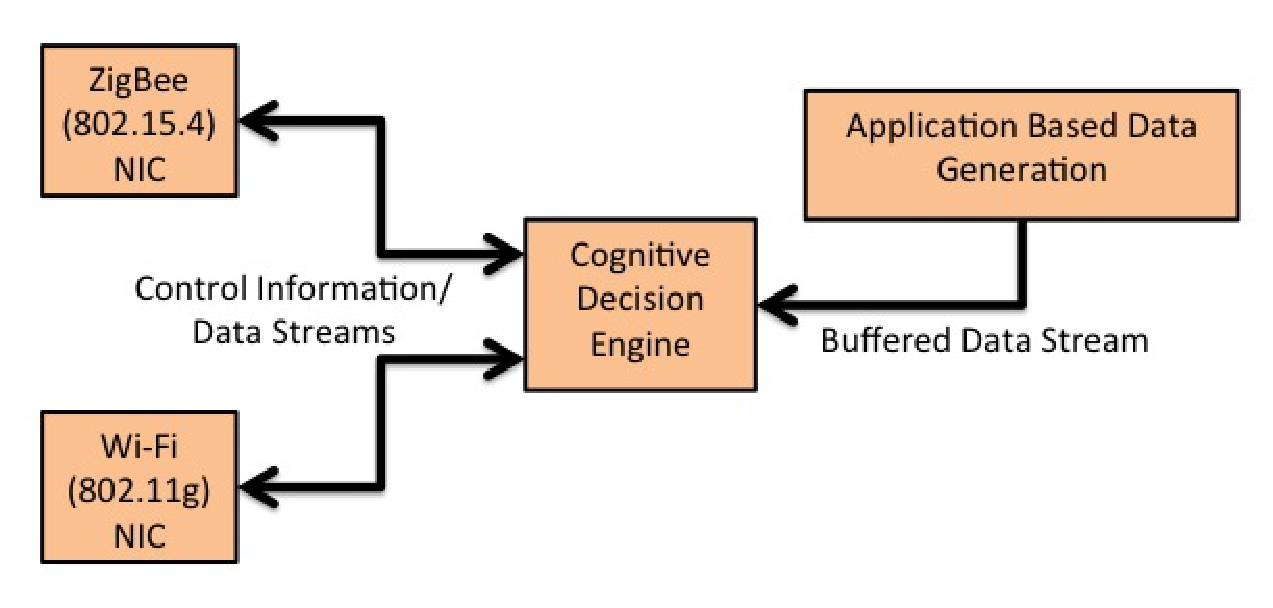
\includegraphics[scale=0.35]{concept_diagram.eps}
\caption{Above is a system concept diagram, showing how network traffic is filtered by a cognitive decision engine to decide which networking interface received data to be transmitted.  The two networking interfaces show here are ZigBee (802.15.4) and Wi-Fi (802.11g).}
\end{center}
\end{figure}

With the advent of smartphones, laptops, netbooks, and portable tablet computers, saving power to extend battery life has been a very active topic within industry. In terms of reducing wireless communications power consumption, an undeveloped approach is to utilize multiple wireless protocols to achieve either power savings while still maintaining acceptable bandwidth for mobile tasks.  Many mobile devices support several wireless protocols such as Wi-Fi, Bluetooth, and 3G.  \cite{six} has examined the benefits of such a combined protocol network.  Their research utilized two networking standards, Bluetooth and Wi-Fi on a laptop base platform.  The actual prototype used complex switching intelligence to examine the advantages of a multiprotocol network and important switching characteristics.  This project experimented with a number of switching policies to study possible power saving methods through reduction in Wi-Fi activity and association times.  The policies used a number of measurement techniques, such as received signal strength indicator (RSSI), transmit power, link quality, and bandwidth capacity.  These measurements were taken to determine appropriate switch timings between wireless protocols\cite{six}.  Bandwidth was the prime metric for their switching calculations.  Though some of the used technics proved tobe unsuccessful, power saving were realized, but at the price a mobility. The main issue with this design was Bluetooth.

For a practical mobile user, Bluetooth is not a logical choice due to its limited range.  Bluetooth was developed as a cable replacement protocol not for multiuser mobility.  For this reason Bluetooth has a very short transmission range making much less effective than the protocol chosen in this paper\cite{thirteen}.  With an infrastructure based network, Bluetooth provides insufficent  mobility seriously limiting users or vastly increasing the needed access points.  Therefore this paper focuses around more applicable protocols for multiple wireless users.  Therefore two protocols were chosen to optimize the power efficiency of the communications system by using a low data rate, low power consumption protocol (ZigBee) for minimal network activity and a high power, high data rate protocol (Wi-Fi) for heavy network traffic. The two wireless protocols provide power efficiency without sacrificing performance relative to a single protocol network, such as Wi-Fi. These protocols will be controlled through an algorithm that monitors the bandwidth of a wireless network, reacting to increases and decreases in network activity, deciding when to switch between protocols. The algorithm monitors the bandwidth of the active radios, and correlates predetermined power consumption to that usage which was accurately determined through preprofiling of the communication interfaces. When the wireless network requires more capacity the algorithm switches Wi-Fi on, and when little to no capacity is needed the algorithm switches Wi-Fi off and ZigBee takes control.  Inherently this dual protocol approach has a power advantage due to the generally limited amount of network activity of mobile devices compared with the duration of their uptime.
This design overcomes the short comings of current single protocol networks by the following:
\begin{enumerate} 
  \item  This project alternates between two complementary wireless standards, without sacrificing mobility and throughput, and decreasing communications power consumption over time. 
  \item  This project intelligently monitors the bandwidth of multiple radios directly and reacts to changes in the bandwidth. 
  \item  This project is power consumption aware. It makes decisions and alternates automatically based on power consumption, bandwidth needs, battery level, etc 
\end{enumerate}

The rest of this paper is organized as follows: In Section II, we present the overall proposed communication system, in section III the power profiling of the communication interfaces, then move on to the implemented prototype, the actual experiments with the hardware, results of the experiments, and finally the conclusion.


\section{Proposed Communication System}
The proposed network uses a hybrid Wi-Fi and ZigBee interface to provide improved power efficiencies on mobile devices.   From a hardware perspective, each node in the network is equipped with a ZigBee and a Wi-Fi radio. The proposed network concept uses two different protocols in an implementation that tries to minimally effect existing mobile infrustructures. In essence, the proposed network implements multi-radio power management that builds upon the already existing wireless infrustructure. Based on the idle power consumption of typical Wi-Fi and ZigBee radios (Table 1), this concept has the potential to realize a large reduction in power consumption for an idle system; however, the actual power savings depends highly on the switching characteristics. The proposed network uses common networking infrastructure and does not require any significant hardware changes. A ZigBee interface, which already exists in many commercial mobile devices, will be installed. ZigBee was designed as a low-power and low-cost interface, and so would be relatively inexpensive to add into many current mobile devices, such as cellphones. 

\setcounter{table}{0}
\begin{table}[h!b!p!]
\caption{Standards Comparision\cite{eight,six,nine,ten,eleven,fourteen}}
\begin{center}
\begin{tabular}{llll}
\hline
Qualifier & Wi-Fi & ZigBee\\
\hline
Data Rate & 54 Mb/s & 250Kb/s\\
Transmission Power Draw & 32-100mW & 0.001-.003mW\\
Idle Power Draw & 0.085W & 0.001-.003mW\\
\hline
\end{tabular}
\end{center}
\label{table1}
\end{table}

\section{Prototype Implementation}
\subsection{System Architecture}
The experimental setup is designed to evaluate the performance of the proposed network and single protocol networks across a variety of network usage conditions.  The architecture of the system is design to abstract both the ZigBee and Wi-Fi interfaces into a single network interface.  The network topology was designed to infrusture based, which is generally more ubiquitous in our internet connected wireless landscape. This proof of concept will only utlize two nodes, a mobile user and a base station or router.  All power savings and adapting protocol switching would be aimed at the mobile user.  Since the base station will not operate on battery power, its consumption can be overlooked.

\begin{figure}
\begin{center}
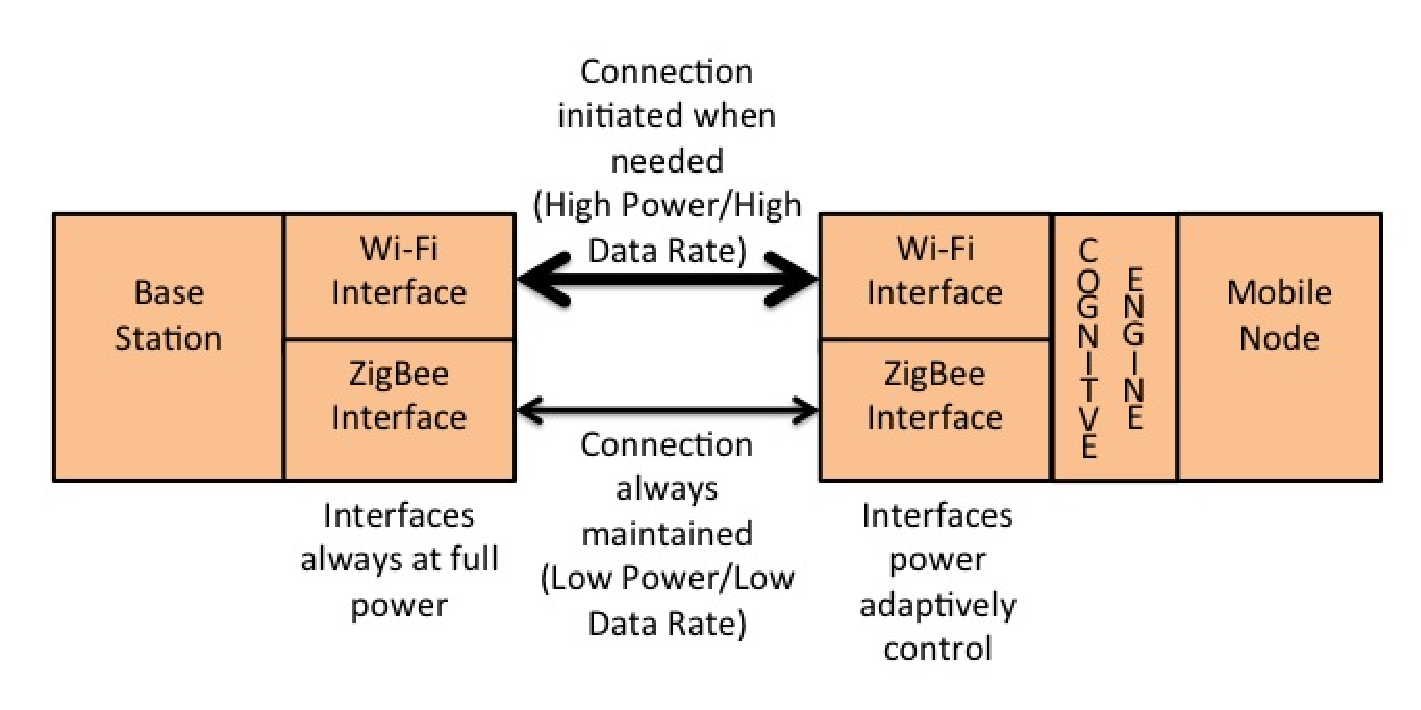
\includegraphics[scale=0.35]{system_diagram.eps}
\caption{Above is a system diagram of the test-bench setup with both external networking interfaces being monitored in real-time.  Both wireless networking interfaces are monitored directly to provide direct information about power consumption, and allow for evaluation of the switching intelligence of the mobile user.}
\end{center}
\end{figure}

Data for the network is generated to represent typical internet usage for a given duration.  This data is then buffered into a single queue, as seen from figure 1, then the switching engine determines which interface will transmit this data.  At all times the ZigBee connection will be maintained and Wi-Fi will be initiated through ZigBee control packets when additional bandwidth is demanded.  Since bandwidth can be relatively difficult to measure from two independant interfaces quickly, the data queue is used instead to measure bandwidth.  Based upon how data built up and left the queue, relative data rates can be determined.

The tests performed by the mobile user represent common tasked performed by mobile devices such as smart phones.  The four primary tasks examined were: large file transfers, small file transfers, web browsing, and purely idle utilization.  All the relevant data is captured by a third data acquisition PC. From this machine, the data is viewed graphically in real-time and exported to a file for analysis. 

%Paragraph about ZigBee
The ZigBee interface was the most difficult to construct due to the limited sophistication of the selected modules.  A simplistic version of TCP was built upon the open-source API xbee-api\cite{fifteen}.  The implementation provided the team with the necessary functionality to maintain links between ZigBee modules and complete bi-directional file transfers.  This was abstracted in the devised switching engine to simplify the interface.


The switching engine itself dynamically alternates between ZigBee and Wi-Fi by using three primary parameters: bandwidth, queue size, and power consumption.  Power consumption was predetermined directly though measurements, and was directly related to transmission usage.  Therefore at any given time, consumption could be determined through bandwidth usage.  This switching engine not only had the ability to direct data flow, but also to initiate connections of the interfaces and reduce their overall power as well.  This switching engine was only developed on the mobile user, the base station or routing unit would remained at full power on both interfaces at all times.

\begin{figure}
\begin{center}
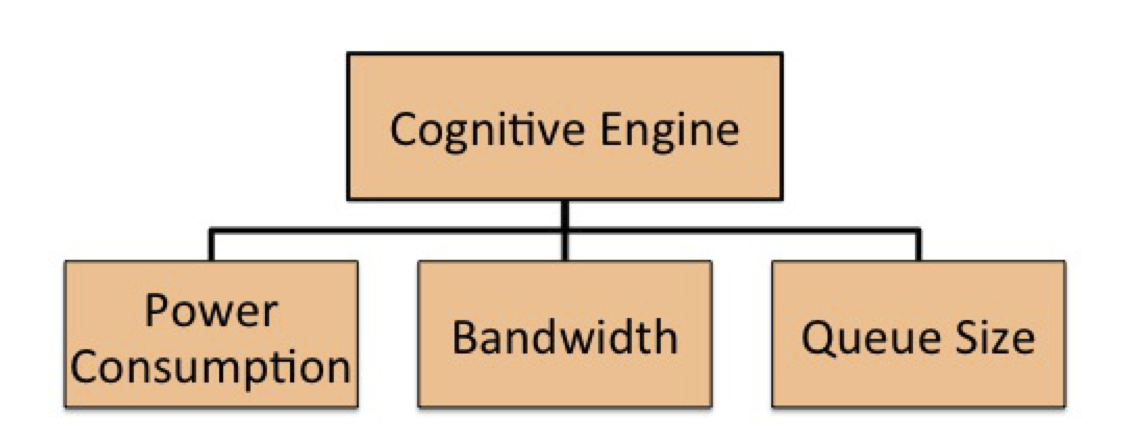
\includegraphics[scale=0.40]{cognitive_para.eps}
\caption{Above shows the breakdown of parameters for the cognitive engine.}
\end{center}
\end{figure}

The base station device effectively acts as a wireless hub which supports both ZigBee and Wi-Fi capabilities, keeping both interfaces active at all times.  The mobile node was responsible for running all network utilization tests and has both wireless interfaces power consumption actively monitored. A third data acquisition machine was originally used for power profiling, and then to measure power usage during experiments.  It utilized a pair of multi-meters to capture detailed power usage of the mobile user.  From this data, energy was determined of the networking interfaces during transmit, receive, and idle modes.  These results can be seen in Table 2.

\setcounter{table}{2}
\begin{table}[h!b!p!]
\caption{Wi-Fi and ZigBee Power Consumption}
\begin{center}
\begin{tabular}{llll}
\hline
Protocol & Action & Power(W) & STD(W)\\
\hline
ZigBee & Tx (Average) & 0.365 & 0.001\\
ZigBee & Rx (Average) & 0.360 & 0.003\\
Wi-Fi & Tx (Average) & 1.454 & 0.005\\
Wi-Fi & Rx (Average) & 1.402 & 0.006 \\
\hline
\end{tabular}
\end{center}
\label{table2}
\end{table}


\subsection{Hardware}
The base station and mobile node are virtually identical hardware components built around the Eee PC 4G Netbook. Each netbook runs a standard version of the Ubuntu 9.10 operating system.  The mobile node uses a Linksys WUSB54G wireless interface adapter for Wi-Fi, and a XBee Series 2 OEM RF Module for ZigBee. The Wi-Fi module uses hand compiled drivers based upon the MadWifi driver. Unless otherwise noted, all Wi-Fi traffic was performed in constantly active mode (CAM), due to that fact that only an ad-hoc wireless can could be utilized for direct connections between netbooks.  Also Wi-Fi connection information is passed through the always on ZigBee connection to primarily reduce the association time of Wi-Fi.

\begin{figure}
\begin{center}
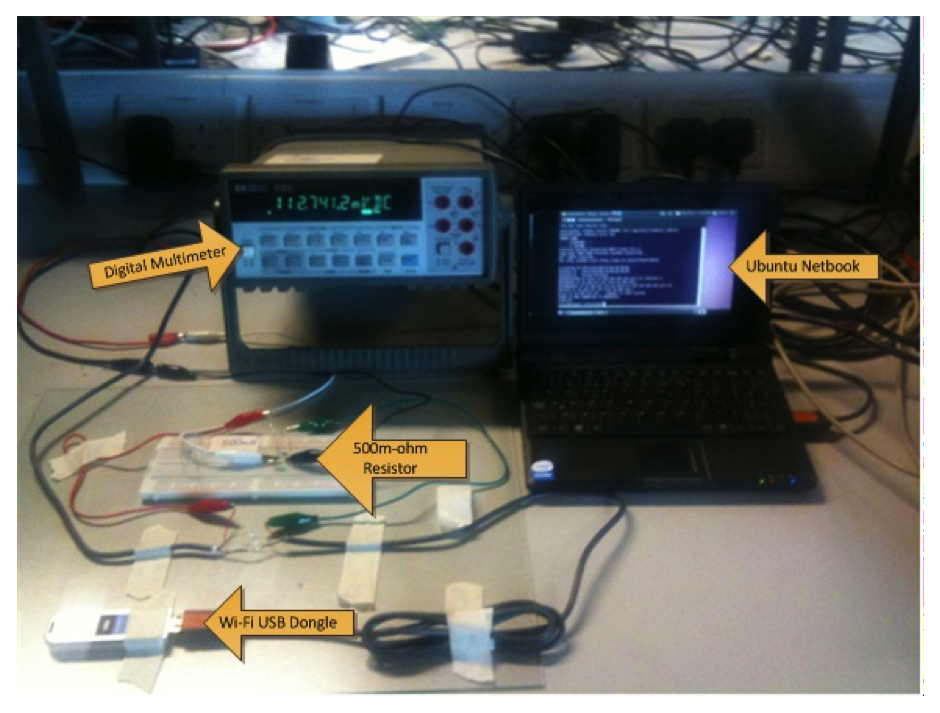
\includegraphics[scale=0.50]{actual_testbench.eps}
\caption{Above is a picture of the actual testbench with only a single multimeter, which is being used to measure the power consumption of the Wi-Fi USB dongle}
\end{center}
\end{figure}

\subsection{Protocol Alternating}
The basic switching process encompasses a start-up process for the higher-level radio that incurs some delay.  The initial switching process can roughly be divided into three parts: connection initiation request, power-up, and connected.  Since the ZigBee channel is always available for communication, data transfer continues until the switch to use the Wi-Fi interface is complete.  Both interfaces are abstracted as a single interface to the operating system.  Data is first buffered into a queue that leads to both interfaces.  Then based upon the amount of data in the queue and how quickly data is added or removed from it determines when to switch between the interfaces occurs.  This switch causes a switch in the queue’s output interface as well, forcing data either through only ZigBee or only Wi-Fi.  These thresholds are based upon measured power characteristics of the physical wireless hardware, the battery level of the node, and application demand.  Since a design requirement was performance transparency, most tasks need to use Wi-Fi to transfer data without considerable delay visible to the user.  Therefore application demand does trump most switching decisions.  Wi-Fi association time was highly focused upon to reduce possible lag during swiches.

\section{Experimental Setup}
\subsection{Experimental Results}

Figure 2 shows an overview of the benefits provided by the proposed network, compared to a Wi-Fi CAM, Wi-Fi PSM, and ZigBee showing both energy and time for a variety of transfer task-base tests. These results represent power consumption per activity.  It is important to note that for most mobile devices that greater that 70\% of device uptime is spent is idle mode.  Through dynamic switching the mobile device can remain out of the power hungry Wi-Fi idle state, and only utilize it when larger data load become queued. Alone the ZigBee interface provides the lowest energy consumption advantage during idle testing, but as soon as any bandwidth intensive task is performed it becomes very power hungry.  Wi-Fi is very power efficient when it comes to data transfer, but when the node becomes idles this is no longer the case.  The proposed network implementation shines in both these cases, expect when the Wi-Fi interface must be maintain for more than 70\% of the device's uptime.  Fortunately for mobile users, 70\% network utilization time is extremely rare.  Overall, when compared with Wi-Fi, the less time the node is actively transferring data the more energy is saved with the proposed network implementation.  The graph below illustrates this fact, extrapolated from measured result of the implemented hardware.

\begin{figure}
\begin{center}
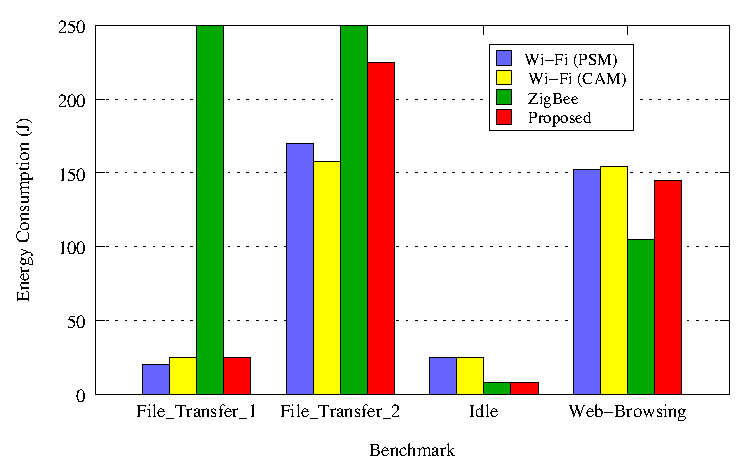
\includegraphics[scale=0.65]{woot.eps}
\caption{The above graph examines the four tests used to evaluate the performance of ZigBee (Green), Wi-Fi PSM (Red), Wi-Fi CAM (Blue), and the proposed combined network (Purple).  File transfer 1 (Far left test) examines the power usage of a transfer that last for 25\% of the test duration.  File Transfer 2 (Second from left) transfers a file for 80\% of the test. The Wikipedia or web-browsing test (second from right) examines common web-browsing usage across a 60 second interval derived from the IMIX web studies of web-browsing habits. \cite{twelve}  The final test (far right) examines power usages for 20 seconds during active no transfers or an idle state.}
\end{center}
\end{figure}

Figure 6 are the results of a 56\% high demand transfer test.  The figure illustrates the power savings over time.  Even at such an intensly data transfer focused test a 10\% decrease in overall power consumption is observed, which as previously explain is an extremely rare usage percentile.  Extrapolating from this data, a saving of 53\% can be saved.  A significant saving.

\begin{figure}
\begin{center}
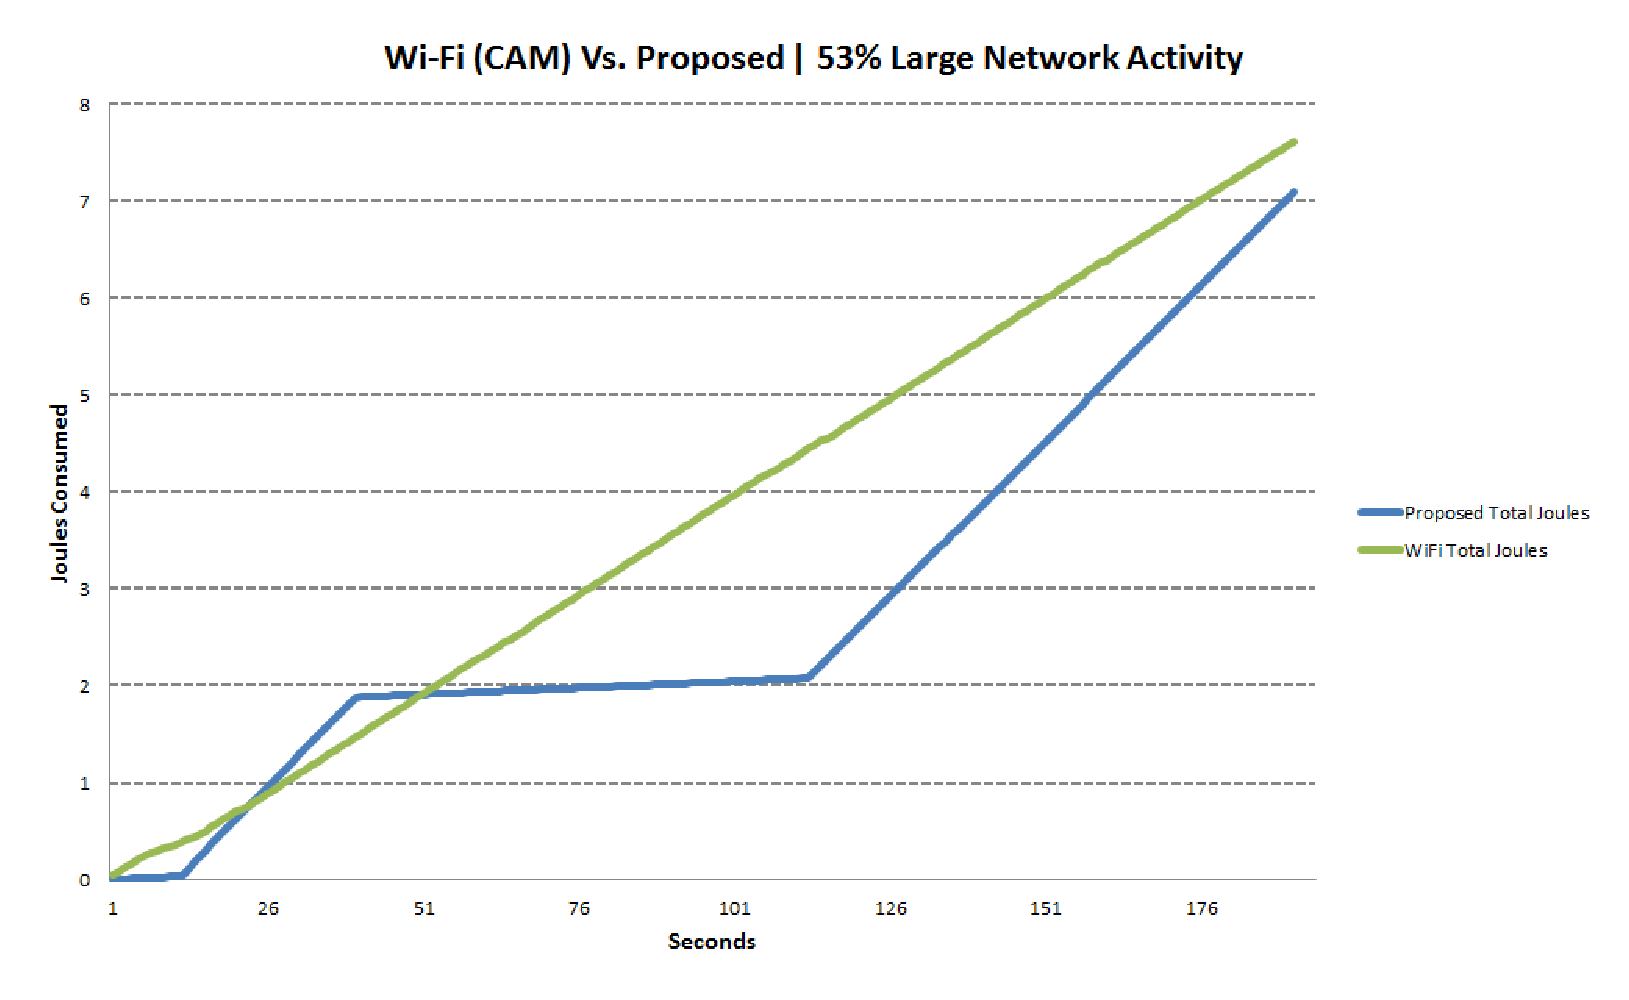
\includegraphics[scale=0.30]{energy_con.eps}
\caption{The above graph compared the amount of energy used over a two minute file transfer test with 53\% activity between a single protocol Wi-Fi (CAM) network and the proposed network.}
\end{center}
\end{figure}


\subsection{Power Measurement Strategy}
The energy measurement setup consists of a HP DAQ Multi-meter data acquisition device connected to a standard Windows XP desktop system with MATLAB. The individual power rails for Wi-Fi and ZigBee are monitored by placing separate 1\%-tolerance 500 mΩ resistors in series with each subsystem’s power supply. Samples are measured at 500 ms intervals, the maximum speed of the multi-meters.  Energy, and not power consumption, is used to show the majority of the results because it captures both the power and time aspects of a particular benchmark. Other components, such as processor, power regulators, memory, display, etc. are not included because, although they are significant power consumers of the mobile device’s battery, they cannot be easily directly measured independently.

Since power consumption monitors do not exists on common network interface cards, it was assumbed that direct real-time measurement and feedback would be impractical.  Therefore a power profile was determined for each network interface cards.  With this profile data, at any data-rate the power being consummed could be calculated in real-time indirectly.  This data was then directly used by our cognitive engine to make determinations when to alternate protocols.  This profile was compared with direct measurements during testing to confirm proper switching and assumed power consumption.


\section{Conclusion}
With such focus in our world today being on mobility, greater efficiencies in communications of these mobile devices must be realized.  For this project was a stepping stone in a new direction in efficiencies of wireless technologies.  The fact alone that off the shelf parts were used with such substantial results only cements the expectation for rapid growth of such a concept.  Combined with the ubiquity of wireless devices and the ever growing market place, multiprotocol systems show tremendous promise for the future.  The applications for multiprotocol systems are far ranging, from large scale communication networks, to house hold appliances and networks.  The greatest advantage is the simplicity and omnipotence of such a concept.  The concept of this multiprotocol approach was proven by the achieved goals of this project. 
The implementation described in this report has successfully achieved the following goals:
\begin{enumerate}
  \item Multi-protocol Network:  The system was able to utilize dual radio protocols to transmit data synchronously
  \item Power Efficiency: The system was able to considerably reduce the communications power consumed compared with a single protocol network
  \item Performance Transparency:   The multiprotocol network performed equally or greater than the a single protocol network as  in terms of throughput
  \item Standard Equipment:  This project only utilized off the shelf part in both nodes of the network
\end{enumerate}

By demonstrating the practical feasibility of this network, a foundation is being established for research and exploration into multiprotocol systems. As standards like WiMax and ZigBee become more common, the practicality for these types of multi-protocol networks will grow. As this project was completed with common equipment, it is only a matter of time before networks like the one described in this report are implemented.  The technology already exists in the market place, it only needs to be recognized and combined.

\section{Future Work}
The goal of this project was to develop a multi-protocol wireless network for the purpose of increasing battery efficency with exisiting wireless standards and hardware.  This paper demonstrates the fessibility and oppurtunity available for such networks, and a simplified hardware model focused around the infrustructure base network would be most appropriate.  Such implementations as ZigBee addons for common access points and routers, again building up the already existing wireless infrustruct proving both economical and effective. 

\bibliographystyle{IEEEtran}
\bibliography{IEEEabrv,LPCN_Conference_Paper_refs.bib}


\end{document}
